% Created by tikzDevice version 0.8.1 on 2015-11-09 20:32:18
% !TEX encoding = UTF-8 Unicode
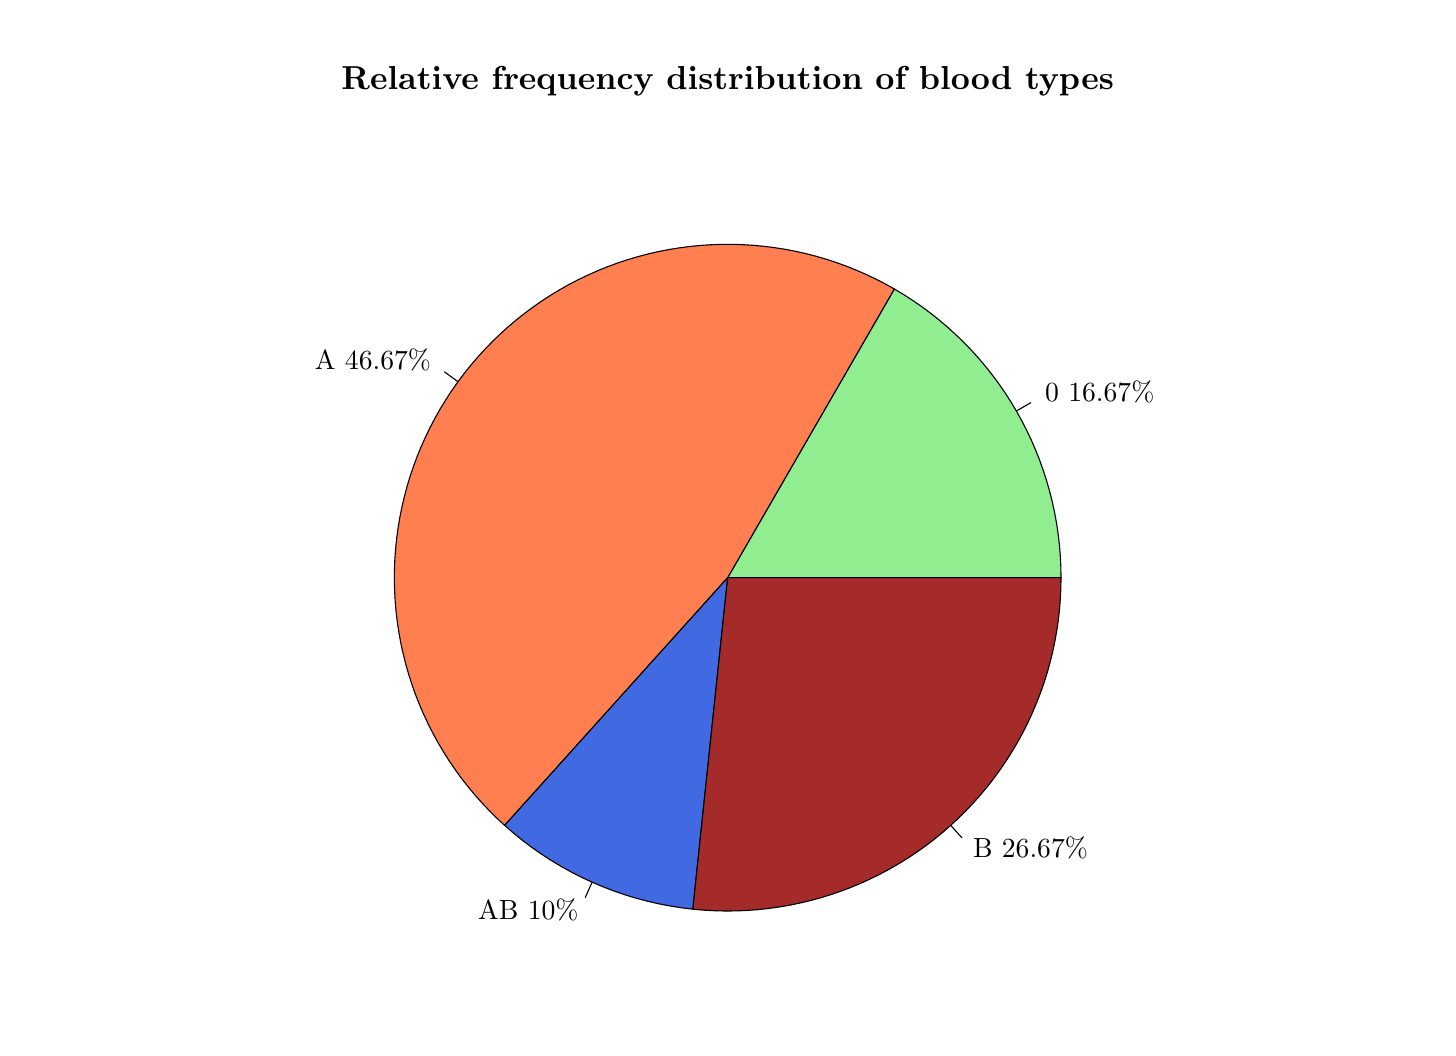
\begin{tikzpicture}[x=1pt,y=1pt]
\definecolor{fillColor}{RGB}{255,255,255}
\path[use as bounding box,fill=fillColor,fill opacity=0.00] (0,0) rectangle (505.89,361.35);
\begin{scope}
\path[clip] (  0.00,  0.00) rectangle (505.89,325.21);
\definecolor{drawColor}{RGB}{0,0,0}
\definecolor{fillColor}{RGB}{144,238,144}

\path[draw=drawColor,line width= 0.4pt,line join=round,line cap=round,fill=fillColor] (373.40,162.61) --
	(373.33,166.55) --
	(373.14,170.49) --
	(372.82,174.41) --
	(372.36,178.33) --
	(371.79,182.23) --
	(371.08,186.11) --
	(370.25,189.96) --
	(369.29,193.78) --
	(368.21,197.57) --
	(367.00,201.32) --
	(365.67,205.04) --
	(364.23,208.70) --
	(362.66,212.32) --
	(360.97,215.88) --
	(359.17,219.39) --
	(357.26,222.83) --
	(355.23,226.21) --
	(353.10,229.53) --
	(350.85,232.77) --
	(348.50,235.93) --
	(346.05,239.02) --
	(343.50,242.03) --
	(340.86,244.95) --
	(338.12,247.78) --
	(335.28,250.52) --
	(332.36,253.17) --
	(329.36,255.72) --
	(326.27,258.17) --
	(323.10,260.51) --
	(319.86,262.76) --
	(316.55,264.89) --
	(313.17,266.92) --
	(252.94,162.61) --
	cycle;

\path[draw=drawColor,line width= 0.4pt,line join=round,line cap=round] (357.26,222.83) --
	(362.47,225.84);
\end{scope}
\begin{scope}
\path[clip] (  0.00,  0.00) rectangle (505.89,361.35);
\definecolor{drawColor}{RGB}{0,0,0}

\node[text=drawColor,anchor=base west,inner sep=0pt, outer sep=0pt, scale=  1.00] at (367.69,226.36) {0 16.67\%};
\end{scope}
\begin{scope}
\path[clip] (  0.00,  0.00) rectangle (505.89,325.21);
\definecolor{drawColor}{RGB}{0,0,0}
\definecolor{fillColor}{RGB}{255,127,80}

\path[draw=drawColor,line width= 0.4pt,line join=round,line cap=round,fill=fillColor] (313.17,266.92) --
	(309.82,268.79) --
	(306.40,270.54) --
	(302.94,272.19) --
	(299.42,273.73) --
	(295.85,275.16) --
	(292.25,276.47) --
	(288.60,277.66) --
	(284.91,278.74) --
	(281.20,279.70) --
	(277.45,280.54) --
	(273.68,281.26) --
	(269.89,281.86) --
	(266.08,282.34) --
	(262.26,282.70) --
	(258.43,282.93) --
	(254.59,283.05) --
	(250.75,283.04) --
	(246.91,282.91) --
	(243.08,282.65) --
	(239.26,282.28) --
	(235.46,281.78) --
	(231.67,281.16) --
	(227.90,280.43) --
	(224.16,279.57) --
	(220.45,278.59) --
	(216.77,277.50) --
	(213.13,276.29) --
	(209.52,274.96) --
	(205.97,273.52) --
	(202.46,271.96) --
	(199.00,270.30) --
	(195.59,268.53) --
	(192.25,266.64) --
	(188.96,264.66) --
	(185.74,262.57) --
	(182.59,260.37) --
	(179.51,258.08) --
	(176.51,255.69) --
	(173.58,253.21) --
	(170.73,250.64) --
	(167.97,247.97) --
	(165.29,245.22) --
	(162.70,242.39) --
	(160.21,239.47) --
	(157.80,236.48) --
	(155.50,233.41) --
	(153.29,230.27) --
	(151.19,227.06) --
	(149.18,223.78) --
	(147.29,220.44) --
	(145.50,217.05) --
	(143.82,213.59) --
	(142.25,210.09) --
	(140.79,206.54) --
	(139.45,202.94) --
	(138.22,199.31) --
	(137.11,195.63) --
	(136.12,191.92) --
	(135.24,188.19) --
	(134.49,184.42) --
	(133.85,180.64) --
	(133.34,176.83) --
	(132.95,173.01) --
	(132.67,169.19) --
	(132.53,165.35) --
	(132.50,161.51) --
	(132.60,157.67) --
	(132.81,153.84) --
	(133.15,150.02) --
	(133.62,146.21) --
	(134.20,142.41) --
	(134.90,138.64) --
	(135.73,134.89) --
	(136.67,131.17) --
	(137.73,127.48) --
	(138.91,123.83) --
	(140.20,120.21) --
	(141.61,116.64) --
	(143.13,113.12) --
	(144.77,109.64) --
	(146.51,106.22) --
	(148.36,102.86) --
	(150.32, 99.56) --
	(152.38, 96.32) --
	(154.54, 93.15) --
	(156.80, 90.05) --
	(159.17, 87.02) --
	(161.62, 84.07) --
	(164.17, 81.20) --
	(166.81, 78.41) --
	(169.54, 75.71) --
	(172.35, 73.10) --
	(252.94,162.61) --
	cycle;

\path[draw=drawColor,line width= 0.4pt,line join=round,line cap=round] (155.50,233.41) --
	(150.63,236.95);
\end{scope}
\begin{scope}
\path[clip] (  0.00,  0.00) rectangle (505.89,361.35);
\definecolor{drawColor}{RGB}{0,0,0}

\node[text=drawColor,anchor=base east,inner sep=0pt, outer sep=0pt, scale=  1.00] at (145.75,237.99) {A 46.67\%};
\end{scope}
\begin{scope}
\path[clip] (  0.00,  0.00) rectangle (505.89,325.21);
\definecolor{drawColor}{RGB}{0,0,0}
\definecolor{fillColor}{RGB}{65,105,225}

\path[draw=drawColor,line width= 0.4pt,line join=round,line cap=round,fill=fillColor] (172.35, 73.10) --
	(175.52, 70.34) --
	(178.79, 67.69) --
	(182.15, 65.16) --
	(185.59, 62.75) --
	(189.12, 60.46) --
	(192.72, 58.29) --
	(196.40, 56.26) --
	(200.14, 54.35) --
	(203.95, 52.57) --
	(207.82, 50.93) --
	(211.75, 49.42) --
	(215.72, 48.05) --
	(219.74, 46.82) --
	(223.81, 45.74) --
	(227.90, 44.79) --
	(232.03, 43.99) --
	(236.18, 43.33) --
	(240.35, 42.82) --
	(252.94,162.61) --
	cycle;

\path[draw=drawColor,line width= 0.4pt,line join=round,line cap=round] (203.95, 52.57) --
	(201.50, 47.07);
\end{scope}
\begin{scope}
\path[clip] (  0.00,  0.00) rectangle (505.89,361.35);
\definecolor{drawColor}{RGB}{0,0,0}

\node[text=drawColor,anchor=base east,inner sep=0pt, outer sep=0pt, scale=  1.00] at (199.05, 39.07) {AB 10\%};
\end{scope}
\begin{scope}
\path[clip] (  0.00,  0.00) rectangle (505.89,325.21);
\definecolor{drawColor}{RGB}{0,0,0}
\definecolor{fillColor}{RGB}{165,42,42}

\path[draw=drawColor,line width= 0.4pt,line join=round,line cap=round,fill=fillColor] (240.35, 42.82) --
	(244.22, 42.47) --
	(248.09, 42.26) --
	(251.97, 42.16) --
	(255.86, 42.19) --
	(259.73, 42.35) --
	(263.60, 42.63) --
	(267.46, 43.04) --
	(271.31, 43.57) --
	(275.13, 44.22) --
	(278.94, 45.00) --
	(282.71, 45.89) --
	(286.46, 46.91) --
	(290.17, 48.05) --
	(293.84, 49.31) --
	(297.47, 50.69) --
	(301.05, 52.18) --
	(304.58, 53.79) --
	(308.06, 55.51) --
	(311.48, 57.34) --
	(314.84, 59.28) --
	(318.14, 61.33) --
	(321.37, 63.48) --
	(324.53, 65.73) --
	(327.61, 68.09) --
	(330.62, 70.55) --
	(333.54, 73.10) --
	(336.38, 75.74) --
	(339.14, 78.47) --
	(341.80, 81.29) --
	(344.38, 84.20) --
	(346.86, 87.18) --
	(349.24, 90.25) --
	(351.52, 93.39) --
	(353.70, 96.60) --
	(355.77, 99.88) --
	(357.74,103.22) --
	(359.60,106.63) --
	(361.35,110.10) --
	(362.98,113.62) --
	(364.50,117.19) --
	(365.91,120.80) --
	(367.20,124.46) --
	(368.37,128.17) --
	(369.42,131.90) --
	(370.34,135.67) --
	(371.15,139.47) --
	(371.84,143.29) --
	(372.40,147.13) --
	(372.83,150.98) --
	(373.14,154.85) --
	(373.33,158.73) --
	(373.40,162.61) --
	(252.94,162.61) --
	cycle;

\path[draw=drawColor,line width= 0.4pt,line join=round,line cap=round] (333.54, 73.10) --
	(337.57, 68.62);
\end{scope}
\begin{scope}
\path[clip] (  0.00,  0.00) rectangle (505.89,361.35);
\definecolor{drawColor}{RGB}{0,0,0}

\node[text=drawColor,anchor=base west,inner sep=0pt, outer sep=0pt, scale=  1.00] at (341.60, 61.65) {B 26.67\%};

\node[text=drawColor,anchor=base,inner sep=0pt, outer sep=0pt, scale=  1.20] at (252.94,339.14) {\bfseries Relative frequency distribution of blood types};
\end{scope}
\end{tikzpicture}
